%======================================================================
\chapter{Related Work} \label{chapter:related_work}
%======================================================================

The contributions of this thesis lie at the cusp between discrete mathematics and bioinformatics. This work involves constructing predictive models to identify important components of genetic sequence data. Modelling biological problems as graphs and other abstract mathematical objects can lead to theoretical results concerning computational complexity and, thus, the ability to find an approximate solution efficiently. In Chapter \ref{chapters:intro} we introduced the central topic of this thesis, motif recognition, gave biological motivation for the study of this problem, and defined several string selection  problems peripheral to this investigation. 

In this chapter, we begin by surveying the theoretical results related to motif-recognition, the {\sc Closest String} problem and variants of the {\sc Closest String} problem.  Each of these problems that we consider is NP-complete and, thus, unlikely to have a  polynomial-time algorithm. Two natural approaches to dealing with the intrinsic computational hardness of these sequence problems are: to consider their parameterized complexity, and to determine if they can be approximated to a reasonable factor in polynomial time.  Prior to this survey, we introduce and define terms from theoretical computer science that will arise in this work, namely those central to the topics of parameterized complexity and approximability. 

In addition to our survey on the important theoretical results related to our study of motif recognition, we give an overview of a short list of programs that detect motifs in synthetic and biological data.  The programs we choose to survey are the ones most well-used or well-studied; the work is either well-cited or frequently used by biologists or bioinformaticians.  
 
\section{Preliminaries}

We provide an overview of the terms and definitions used in this thesis, and a detailed review of parameterized complexity and the theory of approximation algorithms.  

\subsection{Notation}

Let $s$ be a string over the alphabet $\Sigma$.  Denote the length of $s$ by $|s|$, and the $j$th letter of $s$ by $s(j)$.  Hence, $s = s(1)s(2)\ldots s(|s|)$.  

Given functions $f$ and $g$ of a natural number variable $n$, the notation $f \asymp g $ ($n \rightarrow \infty$) is used to express that $$\lim_{n \rightarrow \infty} \frac{f(n)}{g(n)} = 1$$ and $f$ is an asymptotic estimation of $g$ (for relatively large values of $n$).  Throughout this work, we will often refer to a short nucleotide sequence of a specific length $k$ as a {\em $k$-mer}.

\begin{definition} {\bf (closest string)}  Given a set of strings $S = \{s_1, \ldots, s_n\}$, each string of length  $\ell$, then a string $s$ is a closest string for $S$ if and only if there is no string $s'$ such that $\max_{i = 1, \ldots, n} d(s', s_i) < \max_{i = 1, \ldots, n} d(s, s_i)$. \end{definition} 

\noindent Similarly, if $s$ is a closest string for $S$ then we define the {\em optimal closest distance} $d$ is equal to $\max_{i = 1, \ldots, n} d(s, s_i)$.  

\begin{definition} {\bf (majority vote string)} We refer to a majority vote string for $S$ as a length-$\ell$ string containing a letter that occurs most often at each position.  A majority vote string -- which we sometimes refer to as the {\em majority string} -- is not necessarily unique. \end{definition}

\noindent There can be up to $|\Sigma|$ unique majority symbols at each position, and up to $|\Sigma|^{\ell}$ distinct majority strings.  When we refer to a randomly selected majority vote string we refer to a string that has the majority symbol at each position with ties broken arbitrarily. 

\subsection{A Brief Introduction to Parameterized Complexity}

Any NP-hard problem $\Phi$ is unlikely to be solved in polynomial time.  Most likely there will be only exponential-time algorithms for $\Phi$.  Fortunately, an exponential-time algorithm can still be efficient if the exponential component of the running time is restricted to parameters that are likely small in practice and the running time is polynomial in all other parameters.  The goal of parameterized complexity is to attempt to restrict the exponential increase of the running time to as few parameters of the instance as possible. 

\begin{definition} A {\em parameterized problem} is a language $L$ contained in $\Sigma^* \times \mathbb{N}$ , where $\Sigma$ is a finite alphabet. The second component is called the {\em parameter} of the problem. \end{definition}

A parameterized problem is specified by three pieces of information: the input, the problem, and the parameters that are designated as fixed.  In classical complexity, tractable problems are defined as those problems solvable by a polynomial-time algorithm.  The analogous concept in parameterized complexity is an algorithm with running time bounded by a function that is polynomial in the size of the input but is allowed to be superpolynomial in the value of the fixed parameters.  

\begin{definition} A problem $\varphi$ is said to be {\em fixed parameter tractable}  with respect to parameter $k$ if there exists an algorithm that solves $\varphi$  in $f(k) \cdot n^{O(1)}$ time, where $f$ is a function of $k$ that is independent of $n$. \end{definition}  

For example, given a graph $G =(V, E)$ with vertex set $V$, edge set $E$, and positive integer $k$, the {\sc Vertex Cover} problem aims to discern where there is a subset of vertices $V_C \subseteq V$ with $k$ or fewer vertices such that each edge in $E$ has at least one of its endpoints in $V_C$.  The {\sc Vertex Cover} problem is NP-complete \cite{GJ} but is fixed parameter tractable since there exist algorithmic solutions that have running time $O(kn + 1.3^k)$ \cite{DF99}. There are several general, sophisticated techniques developed for the design of efficient parameterized algorithms, including the bounded search tree method, reduction to the problem kernel, and perfect hashing \cite{DF99}.   A problem that is fixed parameter tractable is said to reside in the parameterized corresponding complexity class FPT.   

Not all problems in NP are believed to be in FPT.  For example, consider the NP-complete {\sc Clique} problem: given an undirected graph $G=(V, E)$ and a positive integer $k$, the aim is to determine whether there is a subset of vertices $C \subseteq V$ of size at least $k$ where each pair of vertices in $C$ are connected by an edge.  {\sc Clique} is believed to be {\em fixed parameter intractable} since it is not known whether it can be solved in time $f(k) \cdot n^{O(1)}$, where $f$ might be an arbitrarily fast growing function only depending on $k$. The best known algorithms for solving clique runs in time $O(n^{o(k)})$ \cite{DF99}.  

In order to characterize those problems that do not seem to admit a fixed parameter efficient algorithm, Downey and Fellows \cite{DF99} defined a {\em fixed parameter reduction}. Let $L, L^* \subseteq \sum^* \times \mathbb{N}$ be two parameterized languages. $L$ {\em reduces} to $L'$ if there are functions $k \rightarrow k'$ and $k \rightarrow k''$ from $\mathbb{N}$ to $\mathbb{N}$ and a function $(x, k) \rightarrow x'$ from $\sum^* \times  \mathbb{N}$ to $\sum^*$ such that:
\begin{enumerate}
\item $(x, k) \rightarrow x'$ is computable in time $k''|x|^c$, for some constant $c$ and
\item $(x,k) \in L$ if and only if $(x', k') \in L'$.
\end{enumerate}

\noindent We note that if $L$ reduces to $L'$ and $L'$ is FPT, then $L$ is FPT.

The goal of parameterized complexity is to determine a finer distinction between problems lying in NP and organize them according to some hierarchy of classes.  The central problem used to provide a model for parameterized non-deterministic computation is the {\sc Weighted Circuit Satisfiability} problem.  The parameterized version of this problem defines an infinite hierarchy of parameterized complexity classes inside NP.  

\begin{definition} A {\em Boolean circuit} $\alpha_n$ with input $x = x_1x_2 \cdots x_n$ of length $n$ is a directed acyclic graph.  The nodes of fan-in 0 are called {\em input nodes} and are labelled from the set $\{0, 1, x_1, \overline{x_1}, x_2, \overline{x_2}, \ldots, x_n, \overline{x_n}\}$.  The nodes of fan-in greater than 0 are called {\em gates} and are labelled either AND, OR, NOT.  A special node is designated the output node.  The {\em size} is the number of nodes and the {\em depth} is the maximum distance from an input node to the output node. \end{definition}

\begin{definition} A gate is said to be {\em large} if the number of inputs to that gate exceeds some specified bound.  The {\em weft} of a decision circuit is the maximum number of large gates on any path from the input variables to the output. \end{definition}

\begin{definition} Given a weft $t$ depth $h$ decision circuit $C$ and a parameter $k$, the {\sc Weighted Weft} $t$ {\sc Depth} $h$ {\sc Circuit Satisfiability (WCS$_{t,h}$)} problem aims to determine whether $C$ has a weight $k$ satisfying assignment. \end{definition}

The set of problems reducible under parameterized reductions to {\sc WCS$_{t, h}$} for any $h$, forms the class called $W[t]$.  The W hierarchy is a collection of computational complexity classes used in the theory of parameterized complexity, classifying computational problems according to their apparent intractability in terms of a parameter other than input size.  

In this thesis we will mainly be interested in the W[1] class, which is considered the lowest intractable class of parameterized complexity.  From a practical perspective, W[1]-hardness gives a concrete indication that a parameterized problem with parameter $k$ is unlikely to have an algorithm that has running time of the form $f(k) \cdot n^{O(1)}$.  XP is the class of all problems solvable in $O(n^{f(k)})$, where $n$ is the size of the input, $k$ a parameter, and $f$ is a computable function independent of $n$. 

The parameterized complexity classes are related to P and NP as follows: $$\mbox{P} \subseteq \mbox{FPT} \subseteq \mbox{W[1]} \subseteq \mbox{W[2]} \subseteq \cdots \subseteq \mbox{W[P]} \subseteq \cdots \subseteq \mbox{XP} \subseteq \mbox{NP.}$$  Parameterized complexity is based on the assumption that FPT $\ne$ W[1], which is very much analogous to the conjecture that P$\ne$NP \cite{DF99}.  


\subsection{A Brief Introduction to Approximability}

Approximation algorithms are used to find approximate solutions to optimization problems and are often associated with NP-hard problems. Since it is unlikely that there can be an efficient, polynomial-time algorithm for solving a NP-hard problem exactly, it is useful to find a reasonable -- though sub-optimal -- solution in polynomial time.  Approximation theory was first introduced  by Johnson \cite{johnson} and since this time and has become a widely-accepted manner to deal with the tractability of hard problems.  When  discussing approximability, the efficiency of the algorithm, the correctness of the solution, and the quality of the approximation are all important concerns. Various measures of approximation quality have been proposed, however, the {\em performance ratio} will be our focus throughout this thesis.

\begin{definition} Let $x$ be an instance of an optimization problem $\pi$ having an optimal solution $opt(x)$. Let $A$ be an algorithm for solving $\pi$, and $A(x)$ the value of the solution produced by $A$ when applied to $x$.  The performance ratio of $A$ with respect to $x$ is $$\max  \{ \frac{A(x)}{opt(x)}, \frac{opt(x)}{A(x)}\}.$$ \end{definition} 

Many results prove the approximation is optimal up to a small constant factor. For example, a $\rho$-approximation algorithm $\mathcal{A}$  for any input $x$ will return a solution whose value will be within a factor $\rho$ times the optimal solution.  For example, the following polynomial-time algorithm is a 2-approximation algorithm for the vertex cover problem: find an uncovered edge and add both endpoints to the vertex cover, until no uncovered edge remains. It is clear that the resulting set of vertices is a vertex cover and is at most twice as large as the optimal one. 

Different optimization problems have different approximation properties relating to the types of approximation algorithms for solving them.  In a $\rho$-approximation algorithm, the value of $\rho$ may be be a function of $|x|$, some other parameter to the problem, or a constant.  A {\em polynomial-time approximation scheme (PTAS)} is an algorithm which takes an instance of an optimization problem and a parameter $\epsilon > 0$ and, in polynomial time, produces a solution that is within a factor $\epsilon$ of being optimal.  Hence, the existence of a PTAS implies that the problem can be approximated within an arbitrarily small factor in polynomial-time.  Not all problems exhibit a PTAS; in fact, any problem hard for the class known as APX does not have a PTAS, unless P=NP \cite{vazirani}. We note that the running time of a PTAS is required to be polynomial in the size of the problem instance for every fixed $\epsilon$ but can differ for various values of $\epsilon$. 

An {\em efficient PTAS (EPTAS)} is an approximation scheme that produces a $(1 + \epsilon)$-approximation in $f(\epsilon) \cdot n^c$ time for some constant $c$.  For example, if $f(\epsilon)$ is $2^{1/\epsilon}$ then such an approximation scheme can be practical even for $\epsilon = 0.1$ and large $n$.  A consequence of W[1]-hardness is that there is no EPTAS for the optimization version of the problem \cite{ct}.

\subsection{A Brief Introduction to Smoothed Analysis}


Smoothed analysis was introduced as an intermediate measure between worst-case and average-case analysis, and is used to explain how many algorithms that are deemed inefficient by worst-case analysis can efficiently find good solutions in practice.  It works by showing that the worst-case instances are fragile to small change; slightly perturbing a worst-case instance destroys the property of it being worst-case.  Spielman and Teng \cite{ST01} analytically showed that the smoothed complexity of the simplex algorithm (with the shadow-vertex pivot rule) for linear programming is a polynomial-time algorithm in practice.  Linear programming is a continuous problem.  The input is a sequence of real numbers: a cost vector and linear constraints.  The smoothing operation adds Gaussian noise with parameter $\sigma$ to each number in the input. The expected running time of the simplex algorithm for such a perturbed instance is polynomial in $1/\sigma$ and the number of input variables. 

Several other papers discuss the smoothed complexity of continuous and discrete problems \cite{BD02,DDM03,Ma08}.  Banderier {\em et al.}\ \cite{DDM03} investigated the concept of smoothed analysis with respect to ordering problems.  They presented and used a {\em partial permutations} perturbation model, where each element of the sequence is independently selected with a given probability $p$ and then a random permutation on the selected elements is performed.  Among other results,  Banderier {\em et al.}\ \cite{DDM03} proved that the expected running time of quicksort on a partial permutation of $n$  elements is $O\left(\frac{n}{p \cdot \log n} \right)$. Manthey and Reischuk investigated the smoothed analysis of binary search trees and prove tight lower and upper bounds of roughly $\Theta(\sqrt{n})$ for the expected height of a binary search tree. 

The smoothed complexity of other string and sequence problems has been considered by Andoni and Krauthgamer \cite{AK}, Manthey and Reischuk \cite{MR05}, and Ma \cite{Ma08}.  Andoni and Krauthgamer \cite{AK} studied the smoothed complexity of sequence alignment by the use of a novel model of edit distance. Their results demonstrate the efficiency of several tools used for sequence alignment, most notably PatternHunter \cite{MTL}. Manthey and Reischuk gave several results considering the smoothed analysis of binary search trees \cite{MR05}.  Ma demonstrated that a simple greedy algorithm runs efficiently in practice for {\sc Shortest Common Superstring} \cite{Ma08}, a problem that has application to string compression and DNA sequence assembly.

\section{Past Work on Motif Recognition}

We have previously introduced the problem of motif recognition and showed the applicability to finding transcription factor binding sites. An obvious method to detect motif instances of length $\ell$ is to generate all possible sequences of length $\ell$ and examine each of these sequences to see if there exists a subsequence in the input that has distance at most $d$ from it.  There are $|\Sigma|^{\ell}$ possible center sequences and each of these sequences can be checked in time $O(mn\ell)$ time. This is essentially one of the first motif-recognition algorithms given by Waterman {\em et al.}\ \cite{WAG84}.  Although this exhaustive algorithm is guaranteed to find a motif set if there exists one, the running time of the algorithm is exorbitantly large and, hence, impractical for even reasonably small motifs.  Nonetheless, due to the applicability of the problem to important problems in biology, it is imperative that efficient algorithms be developed for it.      Numerous algorithms have been developed to solve specific instances of the problem, including PROJECTION \cite{BT02}, Winnower \cite{PS00}, pattern driven approaches \cite{SLC04}, MITRA \cite{EP02}, PSM1 \cite{RBH05}, PMSprune \cite{JBR07}, the Voting algorithm \cite{CL05}, MEME \cite{BE95}, VAS \cite{CL06}, RISOTTO \cite{PCMS06}, Weeder \cite{PMMP04} and several others.  We will discuss several of these algorithms in more detail in this section.     

\subsection{Theoretical Results}

A crucial first step in the study of the complexity of motif recognition is the determination of whether the problem lies within the complexity class NP.  The {\em Verify Algorithm} demonstrates that the problem can be solved in non-deterministic polynomial time.  The algorithm aligns the supposed center string with all possible length-$\ell$ substrings in the set of the input sequences, counts the number of matching positions, and returns whether or not it is a valid center string.  Hence, the complexity of the algorithm is $\Theta(nm\ell)$.  

\begin{algorithm*}[h]
\caption{Verify Algorithm}
\begin{algorithmic}
\STATE {\bf Input:} A set $S = \{S_1, S_2, \ldots, S_n \}$ of $n$ length $m$ sequences, a string $s \in \Sigma^{\ell}$, and parameter $d$.
\STATE {\bf Output:} A boolean value indicating whether there is a length $\ell$ substring in each sequence in $S$ with distance at most $d$ from $s$.
\STATE Let $\alpha \leftarrow$ true.
\STATE {\bf For} $i = 1, \ldots, m$:
\STATE \hspace{5mm} Let $\alpha_i \leftarrow$ false.
\STATE \hspace{5mm} {\bf For each} length $\ell$ substring $s_i$ of $S_i$:
\STATE \hspace{10mm} {\bf If} $d(s_i, s) \leq d$ {\bf then} $\alpha_i =$  true. 
\STATE \hspace{5mm} {\bf If} $\alpha_i$ is false {\bf then} $\alpha =$ false.
\STATE Return $\alpha$.
\end{algorithmic}
\end{algorithm*}

After the verification that the problem is in NP, the next aim is to determine whether it is in P or NP-complete.  Unfortunately, the problem is known to be NP-complete, and unlikely to be solved in polynomial-time, unless P = NP \cite{FL97}. There are two natural approaches to investigate the computational intractability of this problem: consider the fixed parameter tractability with respect to the problem parameters ({\em i.e.} $\ell$, $n$, or $d$), and consider the ease with which it can be approximated with reasonable accuracy and efficiency. 

In \cite{ESW03} and \cite{FGN06} it is shown that the problem is W[1]-hard even if all three of $n$, $d$ and $\ell$ are fixed and the alphabet is unbounded. Smith demonstrated the problem is W[1]-hard when $m$ and $\ell$ are parameters and $|\Sigma|$ is unbounded \cite{asmith}.   On the other hand, if $|\Sigma|$ and $\ell$ are both parameters, then the problem becomes fixed-parameter tractable since we can enumerate and check all the $|\Sigma|^{\ell}$ possible center strings.  

If the strings are long, which is often the case in practical applications, then it makes more sense to assume that the number of sequences $n$ or the degeneracy $d$ are parameters.  In \cite{FGN06} it is shown that the problem is W[1]-hard with parameter $n$, even if the alphabet is binary.  Recently, Marx \cite{marx} demonstrated that motif recognition is W[1]-hard with respect to the parameter $d$ or with the combined parameters $d$ and $n$, even if the alphabet is binary.   Table \ref{tab:fpt_motif_recogniton} summarizes these results. Further, Marx \cite{marx} presented two algorithms that aim to be efficient for small fixed values of $d$ and $n$: for some functions $f$ and $g$ and size of the input $k$, the algorithms have running times $f(d) \cdot k^{O(\log d)}$ and $f(d, n) \cdot k^{O(\log \log n)}$, respectively.  The second algorithm is based on connections with extremal combinatorics of hypergraphs.  

Lastly, Ma and Sun \cite{MS08} gave a new algorithm with improved time complexity $O((16|\Sigma|)^d \cdot nm^{\lceil \log d \rceil  + 1})$.  Smith gave some results considering membership in the W-Hierarchy beyond the W[1] parameterized complexity class \cite{asmith}; however, we will restrict interest to the W[1]-hardness throughout this thesis. In addition, he presented the first fixed parameter tractable variant not parameterized with the alphabet size \cite{asmith}.  
 
\begin{table}[h]
\begin{center} 
\begin{tabular}{ l  c c c }
	\hline
  Parameter(s) 		& $|\Sigma|$ is constant 		& $|\Sigma|$ is a parameter		& $|\Sigma|$ is unbounded  \\
  \hline
  $d$					& W[1]-hard	\cite{FGN06}		& W[1]-hard	\cite{FGN06}			& W[1]-hard \cite{ESW03,FGN06} 				\\
  $d, n$				& W[1]-hard	\cite{FGN06}		& W[1]-hard	\cite{FGN06}			& W[1]-hard \cite{ESW03,FGN06} 				\\
  $n$					& W[1]-hard	\cite{FGN06}		& W[1]-hard \cite{FGN06}			& W[1]-hard \cite{ESW03,FGN06}				\\
  $\ell$					& FPT (trivial)							& FPT (trivial)								& W[1]-hard \cite{ESW03,FGN06}				\\
  $\ell, d, n$			& FPT (trivial)							& FPT (trivial)											& W[1]-hard \cite{ESW03,FGN06}				\\
  $\ell, m$			& FPT (trivial)							& FPT (trivial)											& W[1]-hard \cite{asmith}				\\
  \hline
\end{tabular} 
\end{center}
\caption{Complexity of motif recognition with different parameterizations}
\label{tab:fpt_motif_recogniton}
\end{table} 

There is a straightforward 2-approximation algorithm for the optimization version of the motif-recognition problem. Li {\em et al.}\ \cite{LMW02} presented a polynomial-time algorithm that achieves a $2 - 2/(2|\Sigma| + 1)$-approximation guarantee for this problem. Lanctot {\em et al.}\ \cite{LLMWZ00} improved upon this result by giving an algorithm that achieves a $(4/3 + \epsilon)$-approximation guarantee in polynomial time, for any small constant $\epsilon > 0$. Ma \cite{ma00} presented a PTAS for the problem.   For a given value of $r$, this PTAS  considers all choices of $r$ substrings of length $\ell$ from the $n$ strings and for each collection of substrings chooses a majority string as the center string.  After all $n^r(m - \ell + 1)^r$ possible collections of substrings are considered, the collection with the smallest maximum (Hamming) distance between the center string and any string in the collection. Smith \cite{asmith} gave a PTAS for the optimization version of the motif-recognition problem where there are no restrictions on the alphabet size, and gave an improvement to the result of Ma \cite{ma00} for the case where the alphabet is binary.  Andoni {\em et al.}\ \cite{AIP} presented a PTAS that achieves a much better time complexity of $O\left(mn^{O(\epsilon^{-2} \log \frac{1}{\epsilon})}\right)$.  Lastly, Ma and Sun \cite{MS08} combined their fixed parameter tractability results to provide a simpler PTAS with time complexity $O\left(mn^{O(\epsilon^{-2})} \right)$.  As suggested by Ma and Sun \cite{MS08}, an important problem that remains open is to find a more efficient approximation algorithm for $\log n < d < \log n / \epsilon^2$.  

In addition, Smith \cite{asmith} presented the idea that the motif recognition optimization problem can be optimized with respect to different objectives, rather than just minimizing $d$.  The different objectives they described are: 
\begin{itemize}
\item Maximize $\ell - d$, which described the similarity between the strings ({\sc Max Closest Substring});
\item Maximize $\ell$ while keeping $d$ constant ({\sc Longest Common Approximate Substring});
\item Maximize $n$, the number of strings ({\sc Maximum Coverage Approximate Substring}).  
\end{itemize}

Smith proved that {\sc Max Closest Substring} is not approximable within $\log n / 4$ in polynomial time (unless P=NP) through a gap preserving reduction the {\sc Set Cover} problem. He also proved {\sc Maximum Coverage Approximate Substring} is APX-hard, and finally, that {\sc Longest Common Approximate Substring} cannot be approximated in polynomial time with performance ratio better than $2 - \epsilon$, for any $\epsilon >0$ unless P=NP \cite{asmith}.  He gave a 2-approximation algorithm for {\sc Longest Common Approximate Substring} and a $|\Sigma|^d$-approximation algorithm for {\sc Maximum Coverage Approximate Substring}.  

Deng {\em et al.}~\cite{DLLM} considered a related string problem, referred to as the {\sc Distinguishing (Sub)string Selection} problem. Given two sets of strings, $S_b$ (bad genes) and $S_g$ (good genes), and two integers $d_b$ and $d_g$ ($d_b \leq d_g$), the aim of the {\sc Distinguishing (Sub)string Selection} problem is to find a (distinguishing) substring $s$ of length $\ell$ that distinguishes the bad strings from good strings -- that is, for each string $S_i \in S_b$ there exists a length-$\ell$ substring $s_i$ of $S_i$ with $d(s, s_i) \leq d_b$ (close to bad strings) and for every substring $t_i$ of length-$\ell$ of every string $T_i \in S_b$, $d(s, t_i) \geq d_g$ (far from good strings). Deng {\em et al.}~\cite{DLLM} presented a PTAS for this problem. Gramm {\em et al.}~\cite{GGN,GGN06} showed the decision version of this problem is W[1]-hard with respect to all combinations of the parameters as given in the problem definition, and gave a fixed parameter algorithm for a very restricted version of the {\sc Distinguishing (Sub)string Selection} problem.

\subsection{Statistical Methods}


We discuss two popular statistical methods for detecting motifs: Multiple EM for Motif Elicitation (MEME) \cite{BE95} and Gibbs sampling \cite{LABLNW}. Other notable statistical methods include CONSENSUS \cite{HS}, the Yeast Motif Detection (YMF) approach \cite{ST03} and Motif Discovery Scan (MDscan) \cite{LBL02}.  Unless otherwise stated, we assume the input to a motif-recognition program is a set of $n$ sequences of length $m$ denoted as $\{S_1, S_2, \ldots, S_n\}$ and the aim is to return is to return a set of length-$\ell$ sequences $\{s_1, s_2, \ldots, s_n\}$, where $s_i$ is a subsequence of $S_i$.

\subsubsection{MEME} 

An {\em Expectation Maximization (EM)} algorithm is a method for finding maximum likelihood estimates of parameters in statistical models, where the model depends on unobserved latent variables. It is an iterative algorithm that alternates between performing an {\em expectation step}, which computes the expectation of the log-likelihood evaluated using the current estimate for the latent variables, and a {\em maximization step}, which computes parameters maximizing the expected log-likelihood found on the expectation step. These estimates of the parameters are used to determine the distribution of the latent variables in the next expectation step \cite{haeseleer}.  

EM can be used to simultaneously optimize the PWM description of a motif \cite{haeseleer}. The weight matrix for the motif is initialized with a subsequence of length $\ell$, plus a small amount of background nucleotide frequencies, for each subsequence of length $\ell$ in the target sequences the probability that it was generated by the motif is calculated (rather than by the background sequence distribution). EM takes a weighted average across these probabilities to generate a more refined motif model. The algorithm iterates between calculating the probability of each site based on the current motif model, and calculating a new motif model based on the probabilities. It can be shown that this procedure performs a gradient descent, converging to a maximum of the log likelihood of the resulting model.

Developed in 1995 by Bailey and Elkan, MEME \cite{BE95} is one of the most popular motif-recognition applications.  The idea is to find an initial motif, then repeat the expectation and maximization steps to improve the motif until it cannot be improved beyond a certain threshold, or the maximum number of iterations has been reached.  MEME uses the PWM motif representation.  

The algorithm has a parameter $\gamma$ that denotes the probability that a sequence is a motif, a motif model $\theta$ that is used to represent the motif, and a background model $\theta_0$ that is used to represent the distribution of the sequences involved.   Both the motif model and the background model are represented by a PWM.  The expectation step computes the probability of finding the site at every position in every sequence based on the given PWM, and in the maximization step, we refine the PWM of the motif given the probabilities for every position and every sequence.  We refine the PWM for $\theta$ by letting the PWM be equal to the probability that a subsequence has a specific nucleotide at a given position.  These probabilities are then normalized so that the entries for a column of the PWM sum to one. Further, with the probability we get from the expectation step, we update the value of $\gamma$.  

For example, suppose we are given the sequence $s = TGATATAACGATC$, and the following PWMs for $\theta$ and $\theta_0$:

\begin{table}[ht]
\begin{minipage}[b]{0.5\linewidth}\centering
\begin{tabular}{|c|c|c|c|c|c|}
\hline
$\theta$ &1&2&3&4&5\\
\hline
A&0.2&0.8&0.1&0.7&0.8\\
\hline
C&0&0.1&0.2&0&0.1\\
\hline
G&0.1&0.1&0.1&0.2&0.1\\
\hline
T&0.7&0&0.6&0.1&0\\
\hline
\end{tabular}
\end{minipage}
\hspace{0.5cm}
\begin{minipage}[b]{0.5\linewidth}
\centering
\begin{tabular}{|c|c|c|c|c|c|}
\hline
$\theta_0$ &1&2&3&4&5\\
\hline
A&0.25&0.25&0.25&0.25&0.25\\
\hline
C&0.25&0.25&0.25&0.25&0.25\\
\hline
G&0.25&0.25&0.25&0.25&0.25\\
\hline
T&0.25&0.25&0.25&0.25&0.25\\
\hline
\end{tabular}
\end{minipage}
\end{table}

As in the expectation step, we consider the subsequence at each possible position of $s$.  Let $p_i$ be the probability that of finding the given subsequence of length 5 at the given position.  Hence, there are 9 possible subsequences and probabilities to consider.

\begin{center}
\begin{tabular}{cccccccccccccc}
 T&\hspace{-4mm}G&\hspace{-4mm}A&\hspace{-4mm}T&\hspace{-4mm}A&\hspace{-4mm}T&\hspace{-4mm}A&\hspace{-4mm}A&\hspace{-4mm}C&\hspace{-4mm}G&\hspace{-4mm}A&\hspace{-4mm}T&\hspace{-4mm}C&\\
 T&\hspace{-4mm}G&\hspace{-4mm}A&\hspace{-4mm}T&\hspace{-4mm}A&\hspace{-4mm}~&\hspace{-4mm}~&\hspace{-4mm}~&\hspace{-4mm}~&\hspace{-4mm}~&\hspace{-4mm}~&\hspace{-4mm}~&\hspace{-4mm}~&$p_1$\\
 ~&\hspace{-4mm}G&\hspace{-4mm}A&\hspace{-4mm}T&\hspace{-4mm}A&\hspace{-4mm}T&\hspace{-4mm}~&\hspace{-4mm}~&\hspace{-4mm}~&\hspace{-4mm}~&\hspace{-4mm}~&\hspace{-4mm}~&\hspace{-4mm}~&$p_2$\\
~&\hspace{-4mm}~&\hspace{-4mm}A&\hspace{-4mm}T&\hspace{-4mm}A&\hspace{-4mm}T&\hspace{-4mm}A&\hspace{-4mm}~&\hspace{-4mm}~&\hspace{-4mm}~&\hspace{-4mm}~&\hspace{-4mm}~&\hspace{-4mm}~&$p_3$\\
~&\hspace{-4mm}~&\hspace{-4mm}~&\hspace{-4mm}T&\hspace{-4mm}A&\hspace{-4mm}T&\hspace{-4mm}A&\hspace{-4mm}A&\hspace{-4mm}~&\hspace{-4mm}~&\hspace{-4mm}~&\hspace{-4mm}~&\hspace{-4mm}~&$p_4$\\
~&\hspace{-4mm}~&\hspace{-4mm}~&\hspace{-4mm}~&\hspace{-4mm}A&\hspace{-4mm}T&\hspace{-4mm}A&\hspace{-4mm}A&\hspace{-4mm}C&\hspace{-4mm}~&\hspace{-4mm}~&\hspace{-4mm}~&\hspace{-4mm}~&$p_5$\\
~&\hspace{-4mm}~&\hspace{-4mm}~&\hspace{-4mm}~&\hspace{-4mm}~&\hspace{-4mm}T&\hspace{-4mm}A&\hspace{-4mm}A&\hspace{-4mm}C&\hspace{-4mm}G&\hspace{-4mm}~&\hspace{-4mm}~&\hspace{-4mm}~&$p_6$\\
~&\hspace{-4mm}~&\hspace{-4mm}~&\hspace{-4mm}~&\hspace{-4mm}~&\hspace{-4mm}~&\hspace{-4mm}A&\hspace{-4mm}A&\hspace{-4mm}C&\hspace{-4mm}G&\hspace{-4mm}A&\hspace{-4mm}~&\hspace{-4mm}~&$p_7$\\
~&\hspace{-4mm}~&\hspace{-4mm}~&\hspace{-4mm}~&\hspace{-4mm}~&\hspace{-4mm}~&\hspace{-4mm}~&\hspace{-4mm}A&\hspace{-4mm}C&\hspace{-4mm}G&\hspace{-4mm}A&\hspace{-4mm}T&\hspace{-4mm}~&$p_8$\\
~&\hspace{-4mm}~&\hspace{-4mm}~&\hspace{-4mm}~&\hspace{-4mm}~&\hspace{-4mm}~&\hspace{-4mm}~&\hspace{-4mm}~&\hspace{-4mm}C&\hspace{-4mm}G&\hspace{-4mm}A&\hspace{-4mm}T&\hspace{-4mm}C&$p_9$\\
\end{tabular}
\end{center}

\noindent Considering the first segment $TGATA$, we calculate the probability $p_1$ as follows: $$p_1 = \frac{\Pr(TGATA | \theta)\gamma}{\Pr(TGATA | \theta)\gamma + \Pr(TGATA | \theta)(1 - \gamma)}.$$  With the probabilities that we get from the expectation set, we calculate $\gamma$ to be equal to $\sum_{\forall i} p_i / 9$ and refine the PWM $\theta$. {\em e.g.}\ the entry for the nucleotide $T$ at position 1 of the refined PWM $\theta$ is equal to: $$\frac{p_1 + p_4 + p_6}{ \sum_{\forall i} p_i}.$$
 
The MEME algorithm has several drawbacks, including the following:  erased input data each time a new motif is discovered since it assumes the new motif is correct, limitation to the two-component case, and extreme pessimism about alignment (which might lead to missed signals).  The most significant drawback of the algorithm is its high time complexity.  

\subsubsection{Gibbs Sampler}


In 1993 Lawerence {\em et al.}\ \cite{LABLNW} presented GibbsDNA, a motif-recognition program that uses a randomized approach to iteratively improve a motif. Gibbs sampling can be viewed as a stochastic implementation of EM. Whereas the latter takes a weighted average across all subsequences (weighted with the current estimate of the probability that they belong to the motif), Gibbs sampling takes a weighted sample from these subsequences. Initially, a motif, represented by a PWM, is selected by choosing one length-$\ell$ subsequence uniformly at random from each of the input sequences.  Let $\theta$ be the motif model, and $\theta_0$ as the distribution of the sequences.  Figure \ref{fig:gibbs_example1} illustrates this initial step of Gibbs sampling.

\begin{figure}[h!]
\begin{center}
 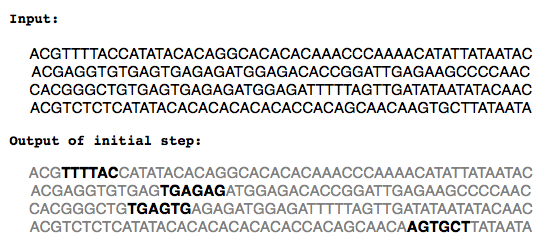
\includegraphics[width=\linewidth]{images/gibbs_example1}
\caption[An example showing the initialization step in Gibbs sampling.]{An example showing the initialization step in Gibbs sampling. The initial step of the Gibbs sampling algorithm chooses a subsequence of a given length from the input sequences uniformly at random.  The subsequences shown in bold are the selected subsequences from this step.}
\label{fig:gibbs_example1}
\end{center}
\end{figure}

At each iteration, the algorithm probabilistically decides whether to add a new site and/or remove an old site from the motif model, weighted by the binding probability for those sites. The resulting motif model is then updated, and the binding probabilities recalculated. Given sufficient iterations, the algorithm will efficiently sample the joint probability distribution of motif models and sites assigned to the motif, focusing in on the best-fitting combinations.  The algorithm repeatedly performs the following steps to iteratively improve the motif:
\begin{enumerate}
\item It selects a sequence $S_i$ at random from the set of input sequences and deletes its length-$\ell$ subsequence.
\begin{figure}[h!]
\begin{center}
 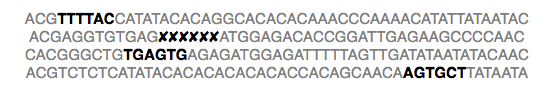
\includegraphics[width=\linewidth]{images/gibbs_example2}
\caption[Illustration of step 1 of Gibbs sampling. ]{Illustration of step 1 of Gibbs sampling.  In step 1 one of the subsequences is chosen randomly and the $\ell$-length subsequence is deleted.}
\label{fig:gibbs_example2}
\end{center}
\end{figure}
\item Next, it defines the PWM $\theta$ based on the remaining length-$\ell$ sequences ({\em i.e.} the subsequences in bold in Figure \ref{fig:gibbs_example2}), and the PWM $\theta_0$ based on the non-motif regions.
\item For each length-$\ell$ subsequence $s_{ij}$ from sequence $S_i$ and starting at position $j$, it calculates $\frac{\Pr(s_{ij} | \theta)}{\Pr(s_{ij} | \theta_0)}$, which is denoted as $score_j$.  
\item The algorithm then lets $\arg \max_{j} score_j$ be equal to $j$. 
\begin{figure}[h!]
\begin{center}
 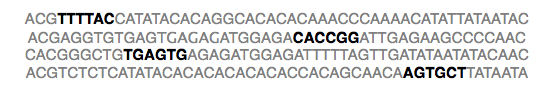
\includegraphics[width=\linewidth]{images/gibbs_example3}
\caption[Illustration of step 4 of Gibbs sampling. ]{Illustration of step 4 of Gibbs sampling.  After the score of each $\ell$-length in sequence $S_i$ is calculated the subsequence that has the maximum score is added, replacing the deleted subsequence in Step 1.}
\label{fig:gibbs_example3}
\end{center}
\end{figure}
\end{enumerate} 

It follows that at each iteration of the algorithm, one of the motif instances is replaced with an improved instance.  When using the Gibbs sampler, a different set of initially selected subsequences will result in a different final set and therefore, to obtain results that are close optimal, the algorithm has to be ran a number of times and the motif instance with the maximum score is returned.  There are several algorithms that use Gibbs sampling as a subroutine.  For example, AlignACE (Aligns Nucleic Acid Conserved Elements) \cite{RHEC} and BioProspector \cite{LBL} are motif-recognition programs that employ a Gibbs sampling strategy.   

\subsubsection{BioProspector}

BioProspector uses Gibbs sampling to search a list of sequences for potential regulatory motifs \cite{LBL}. Gibbs sampling first initializes the motif matrix using length-$\ell$ subsequences that are randomly selected from the input; then, it samples from all length-$\ell$ subsequences in the input sequences to update the PWM. The probability of selecting a length-$\ell$ subsequence is proportional to the likelihood of generating it from the current motif matrix over the likelihood of generating it from the non-motif background. The motif matrix is updated until convergence, or until a certain number of sampling iterations has been reached. BioProspector has several significant improvements compared to GibbsDNA. It uses a Markov model estimated from all promoter sequences in the genome to model adjacent nucleotide dependency and improve motif specificity. It also adopts two thresholds to allow each input sequence to contain zero or multiple copies of the motif \cite{LBL}.

\subsubsection{MDScan}

MDScan \cite{LBL02} is a motif-discovery program that combines two widely adopted motif search strategies: word enumeration \cite{bussemaker,ST03,vanHelden,vilo} and position-specific weight matrix updating \cite{BE95,HHS90,LBL}.  It has been shown to detect longer motifs with a greater number of degenerate positions, however, it is unable to detect $(15, 4)$-motifs with adequate accuracy \cite{LBL02}.
  
\subsubsection{CONSENSUS}

CONSENSUS is a greedy algorithm that is based on a matrix consensus of overrepresented motifs in a set of sequences, coupled with a phylogenetic assessment of the statistical robustness of this motif \cite{HS}.

\subsubsection{The YMF Approach}

The Yeast Motif Detection (YMF) approach calculates the $z$-score for each oligomer occurring in the data set and has been shown to successfully detect motifs in yeast genomes. The success of YMF in detecting transcription factor binding sites in the yeast genome is due to the simplicity of the problem: the short motif length and small number of degenerate positions. Unfortunately, YMF is not suitable for detecting motifs where the length is large and the number of degenerate positions is significant.

\subsection{Combinatorial Methods}

Combinatorial approaches to motif-recognition use the motif model given in Definition \ref{def:combinatorial_motif}. The aim of these methods is to solve progressively weaker and more computationally challenging problems with superior accuracy and efficiency. For example, WINNOWER, which was developed in 2000, was capable of solving of solving the $(15,4)$-motif problem with 20 sequences, each of which had length at most 700 bp \cite{PS00}, whereas PSM1, which was developed in 2005, was able to solve the $(18, 6)$-motif problem with 20 sequences, each of which has length at most 1000 bp, with increased accuracy. We will describe the following three combinatorial approaches to motif recognition in detail: SP-STAR, WINNOWER \cite{PS00}, and PROJECTION \cite{BT02}. 

\subsubsection{SP-STAR}
 
SP-STAR, developed by Pevzner and Sze \cite{PS00}, does an enumerative search but only over a restricted search space defined by the data instead of the entire space. First, a set of subsequences is chosen as the initial motif, and then the best possible motif is obtained by employing a local improvement heuristic that uses scoring function that evaluates the strength of the motif. Given a set of length-$\ell$ sequences $\{x_1, x_2, \ldots, x_n\}$, we define $SPscore$ as $\sum_{i, j} d(x_i, x_j)$.   We summarize SP-STAR in the following steps:
\begin{enumerate}
\item Let $X$ be the set of all length-$\ell$ subsequences in the $n$ input sequences $\{S_1, \ldots, S_n\}$.
\item For any length-$\ell$ sequence $x \in X$ chosen uniformly at random, do the following:
\begin{enumerate}
\item\label{step1} Find the set of $n$ length-$\ell$ sequences $\{s_1, \ldots, s_n\}$ such that $s_i$ is contained in $S_i$ for all $i$, and $d(x, s_i)$ is minimized. 
\item\label{step2} Let $x$ be a sequence that contains the alphabet symbol that occurs most frequently at each position and with ties broken arbitrarily. 
\item Repeat steps \ref{step1} and \ref{step2} until $SPscore$ of $\{s_1, \ldots, s_n\}$ cannot be further improved. 
\end{enumerate}
\end{enumerate}

The algorithm is rerun a number of times and the set of sequences that minimizes $SPscore$ is returned.  Further, the authors suggest that the local improvement steps ``may take a long time'' \cite{PS00} and therefore, should only be performed on a fraction of the best initial sets of sequences. Nonetheless, the number of sequences to be searched is approximately ${\ell \choose d} 3^d$. SP-STAR was successful in finding $(15,4)$-motif instances in data sets containing 20 sequences, each of which has maximum length 700 but failed to have reasonable accuracy when the sequence length exceeded 700 \cite{RBH05}. 

\subsubsection{WINNOWER}

WINNOWER is a simple graph-theoretic approach that represents a motif instance as a clique\footnote{A clique is a graph in which every pair of vertices is joined by an edge.}. WINNOWER first constructs a graph $G(V, E)$ by creating a vertex for every subsequence of length $\ell$ occurring in the input and adding an edge between all pairs of vertices corresponding to subsequences that are distance $2d$ apart and occurring in different input sequences. Now the problem of finding a $(\ell, d)$-motif corresponds to finding a clique of size $n$.  However, clique finding is NP-complete \cite{GJ} and therefore, WINNOWER proposes a method to detect and delete spurious edges to reveal sets of vertices whose corresponding subsequences are possible motif instances \cite{PS00}.    We note that $G$ is a $n$-partite graph\footnote{A $n$-partite graph is a graph where the vertices can be partitioned into $n$ disjoint sets and there are no edges between vertices in the same set.}. 

We define a vertex to be a {\em neighbour} of a clique $C$ if it is connected to every vertex in $C$, and a clique to be {\em extendable} if it has at least one neighbour in each of the $n$ partitions of $G$.  The algorithm is based on the observation that every edge in a maximal $n$-clique belongs to at least ${n-2}\choose{k - 2}$ extendable cliques of size $k$.  An edge is referred to as {\em spurious} if it does not belong to any extendable clique of size $k$.  WINNOWER then iteratively deletes spurious edges for increasing values of $k$ with the idea that only extendable cliques remain.

When $k = 1$, a vertex $u$ is a neighbour of a vertex $v$	if $(u, v) \in E$.  Every vertex that does not contain at least $n - 1$ neighbours is deleted (since it certainly cannot be in a clique of size $n$).  For $k = 2$, a vertex $u$ is a neighbour of an edge $v, w$ if $v$, $w$, and $u$ form a triangle.  Therefore, any edge that does not have $n - 2$  neighbours that are from different partitions is deleted from $G$.  For $k > 2$, WINNOWER relies on the observation that for any clique of size $n$, there are $n \choose k$ extendable cliques with $k$ vertices and thus, every edge on a $n$-clique must belong to at least ${n - 2}\choose{k - 2}$ extendable cliques of size $k$.  Any edge that is not contained in the required number of extendable cliques is deleted.  

\begin{figure}[h]
\begin{center}
 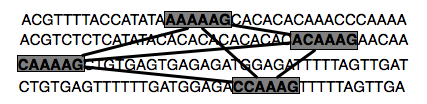
\includegraphics[width=\linewidth]{images/winnower}
\caption[An example showing a clique, which does not correspond to a motif set, in the graphical representation of the input used by WINNOWER. ]{An example showing a clique, which does not correspond to a motif set, in the graphical representation of the input used by WINNOWER. Let $\ell = 6$, $d = 2$, and $n = 4$.  In this example, we have set of sequences where each pair of sequences has distance at most $2d$ but there does not exist a length-$\ell$ sequence that has distance at most $d$ from each of the sequences in the set.}
\label{fig:winnower}
\end{center}
\end{figure}


One of the pitfalls of WINNOWER is that it does not actually report any motifs; it is only concerned with identifying cliques containing $n$ vertices.  Not all cliques correspond to valid motifs (according to the definition of Pevzner and Sze \cite{PS00}) and therefore, further analysis is required to distinguish cliques corresponding to valid motifs from those that are not.  See Figure \ref{fig:winnower} for an example of a set of sequences that corresponds to a clique but not a motif. 

The running time of the algorithm is $O(N^{2d + 1})$, where $N=nm$, and $m$ is length of the input sequences. The algorithm performs better than SP-STAR with the same data sets. However, due to the large number of spurious edges, the running time is prohibitively large and grows very rapidly as the motif strength weakens or subsequence length or number increases \cite{LSB04}.   

There have been many motif-recognition programs that have extended WINNOWER since its initial development.  In 2003, Liang {\em et al.}\ \cite{LSB04} presented cWINNOWER, which is essentially the WINNOWER algorithm with added constraints on the graph construction whose purpose is to reduce the number of spurious edges in the initial graph. Sze {\em et al.}\ \cite{SLC04} extended the graph formation of WINNOWER \cite{PS00}; they formulate the motif-finding problem as the problem of finding large cliques in $k$-partite graphs, with the additional requirement that there exists a string $s$ that is close to every motif instance.  Yang and Rajapakse \cite{YR04} adopted a graph formulation similar to Pevzner and Sze \cite{PS00}, then use a dynamic-programming approach to search for each clique of size $n$. The motif instances and center strings are then derived during the clique finding. Finally, a rescanning of the data set is done with the center string or the motif in order to find motif instances with Hamming distance less than or equal to $d$ from the center string. Lastly, PRUNER \cite{pruner} again uses the same graph formulation as Pevzner and Sze \cite{PS00} but deciphers between the cliques corresponding to a motif by further restricting the criteria for deleting an edge.  All of these algorithms -- cWINNOWER, the work of Sze {\em et al.}\ \cite{SLC04}, the work of Yang and Rajapakse \cite{YR04}, and PRUNER --  suffer from the limitation that an exorbitant amount of  time and space is needed to obtain decent results \cite{LSB04,pruner,SLC04,YR04}.

\subsubsection{Random Projection}

In 2002, Buhler and Tompa developed PROJECTION, an algorithm based on random projections \cite{BT02}.  Assume that we have an $(\ell, d)$-motif problem, and $s_m$ denotes the motif that we are interested in detecting.  PROJECTION considers all length-$\ell$ subsequences in the input set, and projects each of these subsequences along $k$ randomly chosen positions, where $k$ is some appropriately chosen value.  Hence, for every subsequence in $S$, generate a $k$-mer $u'$ that is a subsequence of $u$ corresponding to the $k$ random positions chosen.  Note that the random positions are the same for all the length-$\ell$ subsequences.  Hence, each length-$k$ subsequence is thought of as an integer.  We group the length-$k$ subsequences according to their integer values ({\em i.e.}\ all the length-$\ell$ subsequences are hashed using the length-$k$ subsequences of any length-$\ell$ subsequence as its hash value).  

If a hashed group has at least a threshold number $\alpha$ of length-$\ell$ subsequence in it then there is a good chance that $s_m$ will have its length-$k$ subsequence equal to the length-$k$ subsequence of this group.  Hence, choosing appropriate parameters is vital to the accuracy and efficiency of PROJECTION.  There are $n(m - \ell + 1)$ length-$\ell$ subsequences in the input and there are $4^k$ possible length-$k$ subsequences.  Therefore, the expected number of length-$\ell$ subsequences that hash into the same bucket is $n(m - \ell + 1)/4^k$. The threshold value $\alpha$ is chosen to be twice this expected value. The value of $k$ has to be chosen small enough so that a significant number of motif instances are grouped together under the projection but large enough so that non-motif instances are not grouped together with motif instances; {\em i.e.}\ $k$ is chosen such that $n(m - \ell + 1) < 4^k$ so that the expected number of random length-$\ell$ subsequences that hashed into the same bucket is less than one. 

The process of random hashing is repeated $r$ times to ensure that that a bucket size of at least $\alpha$ is observed at least more than once.  The value of $r$ is defined with respect to several other values which we now define. The probability $p$ that a given motif instance hashes to the planted bucket is equal to ${{{\ell - d}\choose{k}}}{{\ell}\choose{k}}$, and it follows that the probability that fewer than $\alpha$ hash into a bucket is $p' = \sum_{i = 1}^{\alpha - 1} {n\choose i} p^i (1 - p)^{\alpha - i}$.  Thus, the probability that fewer than $\alpha$ hash into a bucket in each of the $r$ trials is equal to $p'^{t}$, which we denote as $P$.  The value of $r$ is equal to $\lceil \frac{\log P}{ \log p'}\rceil$.  In the original paper of Buhler and Tompa, a value of $0.05$ is used for $P$ \cite{BT02}.  In the final step of the algorithm, the sets of length-$\ell$ subsequences that pass the threshold are collected and processed to obtain the motif sequences that are returned.

\subsubsection{The Voting Algorithm}

In 2005, Leung and Chin \cite{CL05} described two algorithms: the Voting algorithm and the Voting algorithm with projection.  The latter is capable of solving challenging motif problems ({\em i.e.}\ the $(9, 2)$, $(11, 3)$ and $(15,5)$ problems), as well as detecting motifs where $\ell$ and $d$ are ``large'' ({\em i.e.}\ the $(20, 7)$ and $(30, 11)$ problems). However, the Voting algorithm (by itself) cannot solve any motif problem when $\ell > 15$ due to heavy time and space requirements \cite{CL05}.  The Voting algorithm with projection uses a similar algorithm as a preprocessing step, then the Voting algorithm is used to recover the motif instances from the set of sequences hashed into the same bucket by projection.  

We give a brief description of the Voting algorithm.  We define a length-$\ell$ sequence $s'$ to be a {\em d-variant} of another length-$\ell$ sequence $s$ if the Hamming distance between $s'$ and $s$ is at most $d$.  We denote all the $d$-variants of a sequence $s$ as $N(s,d)$.  Note that if $s_m$ is a motif then $s_m$, along with all the instances are contained in $N(s_m, d)$.  Then for each length-$\ell$ subsequence $s_i$ in the input sequences gives a vote to each of the sequences in $N(s_i, d)$. Further, each length-$\ell$ sequence can get at most one vote from each of the $n$ input sequences, which ensures that a motif $s_m$ gets exactly $n$ votes. Although the basic Voting algorithm performs better than the basic enumeration algorithm, the required amount of space grows exponentially with $d$, rendering it impractical for reasonable sized values of $\ell$ and $d$.   

\subsubsection{Pattern Branching}

Pattern Branching is a local search algorithm that begins from subsequences that appear in the set of input sequences and systematically alters these initial sequences by changing one letter at a time in order to search for the center sequence \cite{patternbranching}.  If $s'$ is any length-$\ell$ sequence then there are ${{\ell}\choose{d}}3^d$ length-$\ell$ sequences that have Hamming distance $d$ from $s'$.  We refer to this set of sequences at the {\em neighbourhood} of $s'$.  One solution to the $(\ell, d)$-motif problem is to consider the neighbourhood of each of the $\ell$-mers in the set of input sequences, score each of the sequences appropriately, and then return the sequence with the highest score.  Since there could be at most ${{\ell}\choose{d}}3^d (n(m - \ell + 1))$ sequences, the space and time requirements of this basic algorithm are prohibitively large.  Nonetheless, there are several algorithms that use this approach \cite{GEW85,WAG84}.

Rather than considering all length-$\ell$ sequences in the neighbourhood of all occurring subsequences in $S$, Pattern Branching  only examines a selected subset of neighbours.  Again, we denote $N(s, d)$ to be all $d$-variants of $s$.  For any input sequence $S_j$ let $d_{min}(s, S_j)$ denote the minimum Hamming distance between $s$ and any length-$\ell$ subsequence of $S_j$.  Lastly, denote $d_{min}(s, S)$ to be $\sum_{j=1}^nd_{min}(s, S_j)$.  For any $\ell$-mer $s_{ij}$ in the input sequence $S_j$ let $BestNeighbour(s)$ be equal to the sequence in $N(s_{ij}, d)$ whose distance $d_min(s_{ij}, S)$ is minimum from all other sequences in $N(s_{ij}, d)$.  Pattern Branching starts from a sequence $s_{ij}$, identifies $s_{ij}^1 = BestNeighbour(s_{ij})$, then identifies $s_{ij}^{k + 1} = BestNeighbour(s_{ij}^{k})$ for all $1 \leq k \leq d - 1$. The best $s_{ij}^d$ among all possible length-$\ell$ subsequences of the input $S$ is output.

 
\subsubsection{Profile Branching}

Profile Branching \cite{PRP} is similar to Pattern Branching; the main difference between the two algorithms is that in the latter, the search space is of {\em motif profiles}, rather than motif sequences. Given an length-$\ell$ sequence $s = s(1), s(2), \ldots, s(n)$, we define the {\em profile} of $s$ to be a $4 \times \ell$ matrix $X(s)$ where each column is defined as follows:


\[x_{i \alpha} = \left\{ 
\begin{array}{l l}
	\frac{1}{2} 	& \quad \mbox{if $s(i) = \alpha$,}\\
  	\frac{1}{6}		& \quad \mbox{otherwise}\\ \end{array} \right. \]

For example, suppose $s = ACCA$ then the motif profile for $s$ is:

\begin{center}
\begin{tabular}{ l | l l l l }
  ~ & 1 & 2 & 3 & 4 \\
  \hline
  A & $\frac{1}{2}$ & $\frac{1}{6}$ & $\frac{1}{6}$ & $\frac{1}{2}$ \\
  C & $\frac{1}{6}$ & $\frac{1}{2}$ & $\frac{1}{2}$ & $\frac{1}{6}$ \\
  G & $\frac{1}{6}$ & $\frac{1}{6}$ & $\frac{1}{6}$ & $\frac{1}{6}$ \\
  T & $\frac{1}{6}$ & $\frac{1}{6}$ & $\frac{1}{6}$ & $\frac{1}{6}$ \\  
\end{tabular}
\end{center}

The algorithm proceeds identically to Pattern Branching but now the sequences in are ranked according to a new score function, which is referred to as the {\em entropy score}.  The Pattern Branching algorithm outperforms the Profile Branching algorithm; however, the latter does not obtain acceptable accuracy when the degeneracy $d$ is large relative to the sequence length $\ell$ \cite{PRP}.   

\subsection{Challenge Problems} \label{challenge_problems_section}

Pevzner and Sze defined the weak motif-recognition problem more concretely by illustrating the limitations of most motif-recognition programs; their results illustrate that although most methods at the time were capable of finding motifs of length 6 with no degeneration, most failed to detect motif instances of length 15 with 4 degenerate positions in a random sample containing 20 sequences, each of which has length 600 bp \cite{PS00}.  Since this problem was defined, many approaches have been developed with the intention of detecting motifs that have a relatively large number of degenerate positions.  Pevzner and Sze coined the phrase ``challenge problems'' to denote problems where the motif degeneracy ({\em i.e.} parameter $d$) is relatively large with respect to the motif length ({\em i.e.} the parameter $\ell$). Since then the phrase has been commonly used and pertains to problems such as the $(12, 3)$, $(15, 4)$, and $(18, 6)$ motif problems as well as many others. 

\subsection{Exact Verses Approximate Algorithms} \label{approximate_solution_section}

Algorithms that are exact are referred to as {\em exhaustive enumeration algorithms} in the literature.  Many exact motif-recognition algorithms are known ({\em e.g.}\ \cite{BJVU98,GEW85,m83,RBH05,ST00,staden,tompa99,vHAC-V}, however, the running times of these algorithms are prohibitively large for any of the challenge problems \cite{BT02}. Exact algorithms are guaranteed to determine the motif and motif instances, whereas, the solution determined by an approximate algorithm is likely to mismatch with the correct motif and motif instances at a number of positions.  We define the {\em success rate} of a given program using the performance coefficient used by Pevzner and Sze \cite{PS00}, Buhler and Tompa \cite{BT02}, and others \cite{CL05,CL06}. 

\begin{definition} ({\bf performance coefficient}) Let $K$ denote the set of $t\ell$ base positions in the $t$ occurrences of the planted motif, and let $P$ denote the corresponding set of base positions in the $t$ occurrences predicted by an algorithm.  The algorithm's success rate is defined as $|K \cap P| / |K \cup P|$.\end{definition}

\noindent A performance coefficient of $0.75$ or greater is acceptable for algorithms not guaranteeing exact accuracy. The success rate of a program will arise when evaluating motif recognition programs. 

Approximate algorithms, such as CONSENSUS \cite{HS}, Gibbs \cite{LABLNW}, MEME \cite{BE95}, and ProfileBranching \cite{PRP} take significantly less time but perform poorly on finding weak motifs; for example (15,4)-motifs are almost completely undetectable using these programs \cite{HHS90}. More recently, there have been a number of programs that are approximate but have decent performance coefficients (over 75\%), including PROJECTION \cite{BT02}, the Voting algorithm \cite{CL05}, PSM1 \cite{RBH05} and PMSprune \cite{JBR07}.  Unfortunately, most programs failed to achieve decent performance coefficients in practical running time for all $(\ell, d)$-motifs we tested.  The details of these experiments will be discussed in depth in later chapters. 

\section{Past Work on the String Selection Problems}

The {\sc Closest String} problem has not only generated a significant amount of research interest in itself, but is also an important subproblem of motif recognition. We will discuss some past results concerning this problem, and later in this thesis, we develop and apply some efficient heuristics for this problem.  

\subsection{The {\sc Closest String} Problem}

Stojanovic {\em et al.}\ \cite{sto} provided a linear-time algorithm for the case $d=1$. There exists a trivial fixed parameter tractability algorithm when $\ell$ remains fixed: simply try all possible $|\Sigma^{\ell}|$ strings.  Gramm {\em et al.}\ \cite{GNR03}  demonstrated that the {\sc Closest String} problem is in FPT when the number of strings $n$ remains fixed.  This parameterized tractability result is based on an integer linear programming formulation with a constant number of variables, and the application of the result of Lenstra \cite{Len}, which states that integer linear programming is polynomial-time solvable when the number of variables remains fixed. Unfortunately, such an integer linear programming formulation is only of theoretical interest since the corresponding algorithms lead to very large running times even when the number of strings is small. When $d$ is fixed, the problem can be solved in $O(nl + nd(d + 1)^d)$ time \cite{GNR03}.  Ma and Sun gave an $O(n |\Sigma|^{O(d)})$ algorithm, which is a polynomial-time algorithm when $d = O(\log n)$ and $\Sigma$ has constant size \cite{MS08}. Most-recently, Wang and Zhu designed an $O(\ell n + nd|\Sigma|^d 2^{3.25d} )$ time fixed parameter algorithm for the {\sc Closest String} problem \cite{WZ}. Chen {\em et al.}\ \cite{CMW} and Zhao and Zhang \cite{ZZ} also improved upon the fixed parameter tractable result of Ma and Sun \cite{MS08}. 

Ben-Dor {\em et al.}\ \cite{BLPR} used a standard linear programming and randomized rounding technique to develop a near-optimal algorithm for large $d$ ({\em i.e.}\ when $d$ is super-logarithmic in the number of strings).  Lanctot {\em et al.}\ \cite{LLMWZ00_v1} gave an approximation algorithm for the {\sc Closest String} problem that achieves a worst case performance ratio of 2.  It is a simple algorithm that constructs an approximate feasible solution in a pure random fashion.  Starting from an empty solution, the algorithm selects at random the next element to be added to the solution under construction.  In subsequent work, Lanctot {\em et al.}\ \cite{LLMWZ00} gave a polynomial-time algorithm that achieves a $\frac{4}{3} + o(1)$ approximation guarantee. Independently, G\c{a}sieniec {\em et al.}\ \cite{GJL} gave a $\frac{4}{3}$-approximation algorithm that uses a similar technique. This improved algorithm is based on a linear programming relaxation of an integer programming model of the {\sc Closest String} problem.   The basic idea consists of solving the linear programming relaxation\footnote{The linear programming relaxation of an integer program is the problem that arises by replacing the constraint that each variable must be an integer in the set $\{0, 1, \ldots, k\}$ by a weaker constraint, that each variable belong to the interval $[0,k]$.} and using the result of the relaxed problem to define an approximate solution to the original problem.   More specifically, Lanctot {\em et al.}\ \cite{LLMWZ00} used randomized rounding for obtaining an integer 0-1 solution from the continuous solution of the relaxed problem; this technique works by letting a Boolean variable $x$ in the linear program be equal to one with probability $y$, where $y$ is the value of the continuous variable corresponding to $x$ in the relaxation of the original integer program.  

Using randomized rounding again, Li {\em et al.}\ \cite{LMW02} proved the existence of a PTAS for this problem.  Unfortunately, the high degree in the polynomial complexity of the PTAS algorithm renders this result only of theoretical interest.  For a given value of $r$, all choices of $r$ subsequences of length $l$ are considered from the $n$ sequences. The algorithm runs in $O(l(nm)^{r + 1})$-time, which is polynomial for any constant $r$.  In 2005, Brejov\'{a} {\em et al.} \cite{brona1} proved the existence of sharper upper and lower bounds for the PTAS on a slight variant of the {\sc Closest String} problem (which they refer to as the {\sc Consensus Pattern} problem) and in 2006, Brejov\'{a} {\em et al.} \cite{brona2} improved upon the analysis of the PTAS for various random binary motif models by showing that there are known ``weak'' instances for which the approximation ratio is $1 + \Theta(1/ \sqrt{r})$ \cite{brona1}, and ``strong'' instances for which the PTAS will be guaranteed to determine the correct answer in efficient time.  Andoni {\em et al.}\ \cite{AIP} gave a novel PTAS that has improved time complexity, and most recently, Ma and Sun \cite{MS08} presented a PTAS with time complexity $O(n^{\Theta(n^{-2})})$, which is currently the best known. 

\subsection{The {\sc Farthest String} Problem}

Lanctot {\em et al.}\ proved the existence of a PTAS for this problem, though the high degree in the polynomial complexity of the PTAS algorithm renders this result only of theoretical interest \cite{LLMWZ00}.  The algorithm is based on the randomized rounding of the relaxed solution of an integer programming formulation.  There have been no improvements on the running time of this PTAS. 

In 2004, Cheng {\em et al.}\ \cite{cheng} gave a $O((|\Sigma|(\ell-d_f)) (\ell-d_f))$ fixed parameter algorithm for the {\sc Farthest String} problem. This fixed parameter tractability algorithm is nearly identical to the algorithm of Gramm {\em et al.}\ \cite{GNR03} for the {\sc Closest String} problem. Most recently, Wang and Zhu gave a $O(\ell n+n d 2^{3.25d_f})$ fixed parameter algorithm for the {\sc Farthest String} problem when the input strings are binary strings \cite{WZ}. 

\section{Summary}

In this chapter, we surveyed some of the important results in motif recognition, the {\sc Closest String} problem, and its variants.  We described two motif-recognition models, including the combinatorial model that was formally introduced by Pevzner and Sze \cite{PS00}.  Since the combinatorial version of this problem was initially described, there has been a plethora of research in developing motif-recognition programs that are efficient and capable of solving computational challenging instances of this problem.  We continue this area of research by developing  an efficient motif-recognition program that is based on a novel weighted graph model, and illustrating how combinatorial and probabilistic insights can be applied to gain even more efficiency and capability in solving computationally challenging instances of motif recognition. 